\chapter{Experimental Design}
\todo{Check number of enrolments, introduce all metadata, and retrieve 
details of cassandra cluster from my computer}

\todo{summary of chapter structure}


\section{University example}
In order to asses the performance of Cassandra when the four solutions are
executed, the experimental \ac{API} was implemented. The \ac{API} was loaded
with entitites belonging to a University keyspace. The University keyspace
designed for the experiments stores details of students and courses in a
university along with the enrolment details of the students. It has three column
families, namley,
\texttt{Student} to store the student details, \texttt{Course} to store course
information and
\texttt{Enrolment} to preserve the relationship between students and the courses
they enrol into. The class diagram for the University keyspace is shown in
Figure~\ref{fexp:ClassDiagram}.

	\begin{figure}[h] \centering
		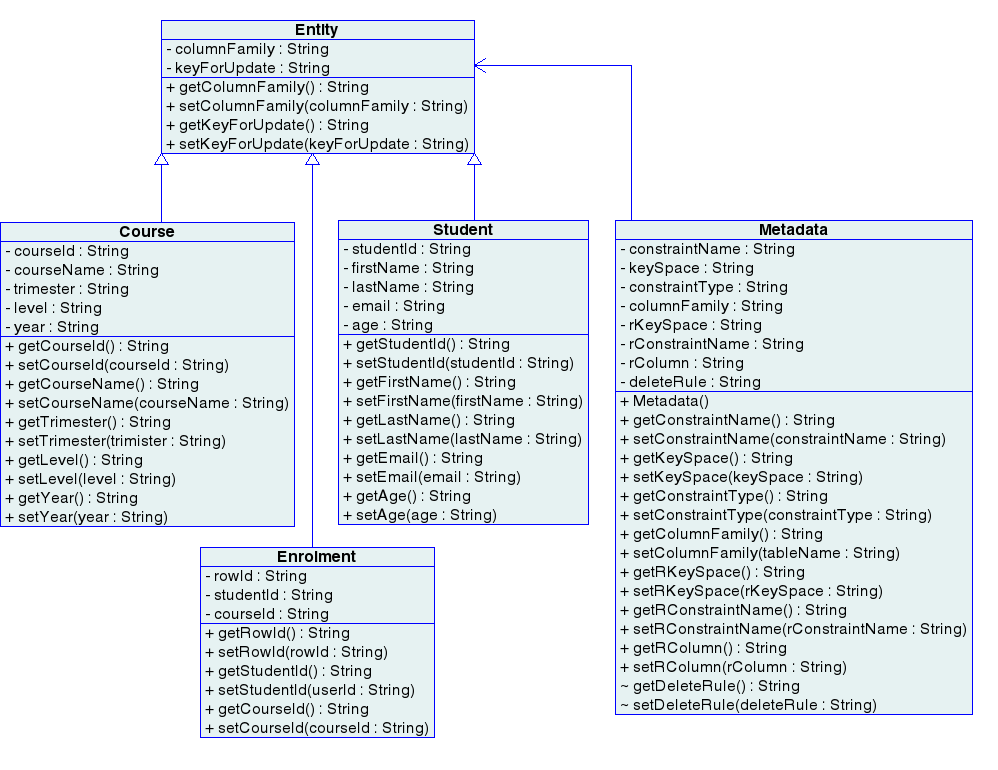
\includegraphics[width=1\textwidth]{./figure/Solutions/classdiagram-experimental.png}
		\caption{Class Diagram for University}\label{fexp:ClassDiagram}
	\end{figure}

The constraints for the keyspace is stored in the \texttt{Metadata} entity.
These constraints are the \ac{PK} and \ac{FK} constraints applicable on each of
the column families in this keyspace. The list of constraints used in ecah of
the solutions are the same and are shown in the following table.
\newline


	
	\newcolumntype{C}{@{\hspace{2.5pt}}>{\scriptsize}c@{\hspace{2.5pt}}}
	\begin{tabular}{CCC CCC CC}
		\toprule
		\bfseries ConstraintName & \bfseries Keyspace & \bfseries ConstraintType &
		\bfseries ColumnFamily & \bfseries RKeyspace & \bfseries RConstraintName &
		\bfseries RColumn & \bfseries DeleteRule\\
		\midrule
		CONST100 & University & P & Student & University & & StudentId &\\
		\rc CONST200 & University & P & Course & University & & CourseId &\\
		CONST300 & University & P & Enrolment & University & & RowId &\\
% 		\hline
% 		\hline
		\rc CONST400 & University & R & Enrolment & University & CONST100 & StudentId
		& CASCADE\\
		CONST500 & University & R & Enrolment & University & CONST200 & CourseId &
		NODELETE\\
		\rc CONST600 & University & F & Course & University & CONST500 & CourseId &
		NODELETE\\
		CONST700 & University & F & Student & University & CONST400 & StudentId &
		CASCADE\\
		\bottomrule
	\end{tabular}
	

The \texttt{ValidationHandler} in each solutions checks these constraints to
validate referential integrity within this keyspace. The entities are loaded
generically by the \texttt{EntityManager} for ecah solution.

In the experiment the number of entities inserted for each column family are
shown in the following table.
	\newline
	\begin{center}
	\newcolumntype{C} {@{\hspace{2.5pt}}>{\scriptsize}c@{\hspace{2.5pt}}}
		\begin{tabular}{CC}
			
			\toprule
			\bfseries ColumnFamily & \bfseries No. of Entities \\
			\midrule
			Student & 1000 \\
			\rc Course & 1000 \\
			Enrolment & 10000  \\
	% 		\hline
	% 		\hline
			
			\bottomrule
		\end{tabular}
	\end{center}

\section{Cassandra cluster}

The environment to deploy cassandra is  an homogeneous cluster conformed by 10
nodes. That is, all 10 nodes have the same characteristics in software and
hardware. These nodes emulate a cloud environment in which each node runs
Cassandra. The characteristics of these nodes are:

\begin{itemize}
  \item Hardware
  \item Software
\end{itemize}




\section{Experimental setup}\label{s:exp:setup}


 The experimentation consists
on performing 100 runs where artificial data is randomly created, updated and
deleted from column famlies in a Cassandra cluster.
On each run, the time required for each operation is recorded in order to assess
the performance of each solution as well as the throughput in terms of
operations per unit of time. Notice that each operation on the artificial data 
is performed in a batch, and entities from each column family are randomly
sorted before any operation takes place. Random sorting is performed in order to
prevent the results to be biased from possible optimization made by Cassandra in
terms of indexes or other criteria.
		
The artificial data is made up of 1000 students, 1000 courses, and 10000
enrolments which are the result of assigning 10 different courses to each
student. Courses are assigned by dividing the number of courses
into 100 groups of 10 courses each, and assigning a group for each student.
Notice that such an assignment involves that X students have the same courses
assigned. The quantity of records to be inserted for each entity was chosen
considering an overall reasonable time for completing the experimentation of all
solutions.
		
The format of the artificial data created is as follows. Student has a
unit-increasing studentId, which is merged into the fields firstName and
lastName as "First Name (studentId)" and "Last Name (studentId)", and trimester
and level are random numbers. Course has a   unit-increasing courseId which is
appended to the prefix "COMP", it also has a composed course name as in
the student (merging id and field). Enrolment contains a unit-increasing rowId, and the
respective foreign keys of student and course.
		
The order of the operations performed on the data is as follows. \textbf{Create}
inserts all the students, courses and enrolments. \textbf{Update} performs
changes on the primary keys of students and courses, and on the foreign keys
of enrolment (the one relative to courses, especifically). Finally,
\textbf{Delete} removes all the students, courses and enrolments.  Notice that
the primary keys in every column family  are different in each run (create,
update, delete) in order to avoid  introducing biases to the results as product
of the tombstone delete paradigm  that Cassandra utilizes. That is, since
Cassandra does not completely  remove the primary keys of the inserted entities
(tombstone delete), reinsertion  using the same primary key might yield faster
times as the key already exists. After  each run, all column families (student,
course, and enrolment) are emptied and  ready for the next run.  The details  of
the \ac{CRUD} operations are explained further in the next sections.
		
	\begin{description}
	
		\item[Create] The create operation inserts all the students, courses and enrolments in
		that precise order due to the nature of the referential integrity constraints
		presented in Section~\ref{s:ed:ri}. The time required to insert all of the
		entities in their respective column families  is recorded. In the Student and
		Course column families, the insertion does not trigger any constraint validation
		as these entities do not contain foreign keys. Contrarily, the insertion of
		enrolments triggers foreign key validation checks on both \texttt{Student} and
		\texttt{Course} column families.
		
		\item[Update] The update operation is performed after the creation of all
		entities.
		First, an attempt to update the primary key of each course is made. This
		triggers constraint validations that result in exceptions thrown as the
		\texttt{DeleteRule} of entity \texttt{Course} is \texttt{NODELETE}. Hence, the
		times recorded for updating the Course column family represent the time required
		to identify a constraint violation and throw the respective exceptions.
					
		Next, the \texttt{Enrolment} column family is updated. In this case, the
		courseId for each enrolment is changed to a different one ensuring that the distribution of
		courses and students remains the same. The update on the enrolment column family
		triggers foreign key validation checks to ensure that the course to which every
		enrolment is being updated actually exists.
					
		Finally, the primary key for each student is updated to a new integer value that
		has never existed in the column family. This operation triggers a cascaded
		update on the \texttt{Enrolment} column family by respectively updating the
		student foreign key in its existing enrolments.
		
		\item[Delete]The deletion of entities occurs first on the Enrolment column family,
		where all of its records are deleted without requiring referential integrity
		checks as this is a child entity. The times are recorded for such operation and
		then all of the entities are reinserted with the same primary keys in order to
		 assess the cascaded delete of students next.
				
		Secondly, all of the students are deleted from their respective column family.
		Given the cascaded delete rule of these entities, the validation handler ensures
		to delete first all of the child entities before deleting an student. Hence, the
		times recorded for this operation measure the time required for performing a
		cascaded delete on the student depedencies in enrolment. Notice that the
		dependencies exist at this point as they will have been reinserted in the
		previous step.
				
		Finally, all of the courses are deleted. Despite the courses having a \texttt{NO
		DELETE} rule, notice that at this point the enrolment column family is empty, so
		courses can be deleted as there are no child dependencies. Thus, the times
		recorded for this operation measure the constraint and referential integrity
		checks as well as the delete operation of the respective entity. After this last
		operation, all column families are emptied but all the primary keys still exist
		due to tombstone. However, the whole keyspace is ready for the next batch of
		operations as the primary keys of all column families will be different.
	
	
	\end{description}		


\section{Performance Measures/Metrics}
Performance of database systems is commonly measured in terms of the
\textit{Response time} and \textit{Throughput}(\todo{cite Demurjian, Berkely}).
Response time refers to the time  a database system takes to process an
operation and produce results to the end user . Measuring response time for a
database operation is similar to a black-box evaluation because it is measured 
without considering the internal functioning  of the database system. According
to (\todo{cite Demurjian}) such an evaluation is ideal for a complete database
system to measure its performance and to give the users details about its 
efficiency and speed in performing operations. In this thesis, response time and
throughput are the measures used to gauge the performance of Cassandra
while referential integrity validation is implemented using the \ac{API}.

Response time for each of the  operations that trigger such a validation from
all the solutions are measured during the experiments. This included the time
involved to access and retrieve metadata for the entities and also the time for
validating referential integrity by the \texttt{ValidationHandler}. The response
time of Cassandra when such validations are not in place is also measured and
considered as a baseline with which to analyse the solutions. Such a comparison 
determines the degree of change in speed of Cassandra when such overheads are
introduced and gives users useful information about how each solution affects
the performance of the database system.

The second performance measure used is \textit{Throughput} which is another
classical and commonly used measure of database performance (\todo{cite
BerkleyDB}).
Throughput measures the number of operations processed by the database system in
a unit of time. In the experiments the throughput for all the operations
triggering referential integrity validation across all solutions is measured as
operations per second.
A single operation stands for each time an entity is inserted or updated or
deleted.
% For example, inserting 1000 students means that 1000 \texttt{insert}
% operations are processed by Cassandra.
Note that only the operations that introduce the referential integrity
validation in Cassandra is measured and thus \texttt{read} operations are not
measured in terms of response time or
throughput.
% These operations
% which trigger referential
% integrity validation for an entity
% namely the \texttt{insert}, \texttt{update}, \texttt{delete} operations are
% were measured in terms of the throughput in the experiments. Throughout commonly
% referes to the number of operations performed

% It has to be noted that the operations are prone to  external factors like
% network latency, bandwidth, network routing, network workload among others which
% typically affect a network consisting of several machines and users. This is
% because the Cassandra cluster used in the experiments is deployed over a
% network that is used by many users concurrently thus exposing the operations to
% such factors. Identifying such factors and analysing them is beyond the scope of
% this thesis and the analysis is strictly in terms of how the metadata storage
% and referential integrity validation affects Cassandra's performance.

The response time and throughput were measured by logging the time involved to
comeplete each operation in all the solutions. 
(\todo{Can quote IBM on this}). Most benchmarks like TPC- cannot be used in our
case as we dont use SQL and neither is Cassandra an OLTP which supports transactions.

Notice that external variables such as network latency, simultaneous processes
in the operating systems of each node, and other variables are not considered
for the analysis of results. Even when they are present, it is expected that
results will not be biased by them. Nonetheless, the experiments will be
performed at night time over a weekend as this is the time where the cluster is
less used, thus reducing the presence of such variables and hence their impact
by biasing the results \todo{or something like that :P}

\section{Summary}
	This chapter has presented the experimental design to evaluate the performance
	of each of the solutions and the api itself using as an example of application
	the toy problem used across this thesis. The experimental design involves
	assessing the performance of the CRUD operations on the different solutions
	proposed for referential integrity. The analysis of results is to be based on
	response time and throughput, two performance indicators that serve as
	guidelines for assessing the tradeoffs between the different solutions
	proposed.
	
	
	The next chapter presents the results and their discussions of the
	experimental design presented in this chapter
 






